% ========== AGERHØNE ==========
\begin{frame}{%
  \begin{minipage}[c]{0.30\textwidth}
    Agerhøne
  \end{minipage}%
  \hfill
  \begin{minipage}[c]{0.45\textwidth}
    \footnotesize
    \textbf{Jagttid:} 16.\ september -- 31.\ oktober*
  \end{minipage}%
  \hfill
  \begin{minipage}[c]{0.15\textwidth}
    \noindent\raggedleft
    
\includegraphics[width=0.5cm, height=0.5cm, keepaspectratio]{Billeder/Ikoner/star.png}%
    \hspace{0.2em}%
    
\includegraphics[width=0.5cm, height=0.5cm, keepaspectratio]{Billeder/Ikoner/star.png}%
    \hspace{0.2em}%
    
\includegraphics[width=0.5cm, height=0.5cm, keepaspectratio]{Billeder/Ikoner/star.png}
  \end{minipage}%
}
  \vspace{0.25em}
  \begin{columns}[T]
    % --- Venstre kolonne: Tekst ---
    \column{0.45\textwidth}
    \setlength{\parskip}{0.45em}
    \tiny
    \RaggedRight
    \textbf{\textit{Perdix perdix}} – lille, buttet hønsefugl med kort hale \par
    \textbf{Udseende:}\\
    \quad – Gråbrun med orangebrunt ansigt og rødbrun hale \\
    \quad – Han har typisk en større mørk hesteskoformet plet på bugen \par
    \textbf{Levesteder:} Åbent agerland med marker, læhegn, skel og enge. \par
    \textbf{Føde:} Ukrudtsfrø, korn og grønt. Kyllinger lever først af insekter. \par
    \textbf{Udbredelse:} Hele Danmark, men i tilbagegang. \par
    \textbf{Træk/standfugl:} Standfugl \par
    \textbf{Forplantning:}\\
    \quad – \textbf{Yngleforhold:} Yngler i hele Danmark \\
    \quad – \textbf{Kønsmoden:} Ca. 1 år \\
    \quad – \textbf{Mono/polygam:} Monogam \\
    \quad – \textbf{Bestandsomsætning:} Hurtig \\
    \quad – \textbf{Kuld:} 10–20 æg \par
    \textbf{*Bemærk:} Lokale jagttider, især vest for Storebælt.
    % --- Højre kolonne: Ét billede ---
    \column{0.52\textwidth}
    \centering
    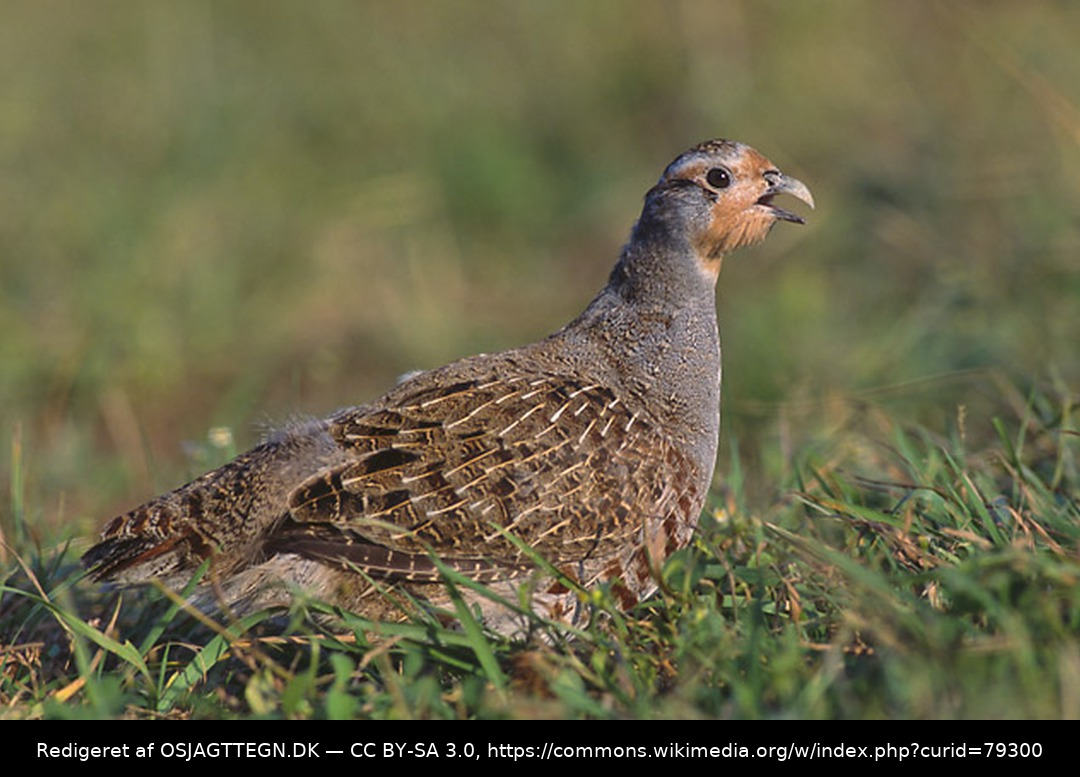
\includegraphics[width=\linewidth, height=7.2cm, keepaspectratio]{Billeder/Dyr/Fugle/Fasanfugle/Agerhøne/agerhoene-01.jpg}
  \end{columns}
\end{frame}